%!TEX TS-program = LuaLaTeX
\documentclass[tikz,border=0.5cm]{standalone}
\usetikzlibrary{shadows} 
\usetikzlibrary{spy} 

\pdfvariable suppressoptionalinfo \numexpr32+64+512\relax

\begin{document}
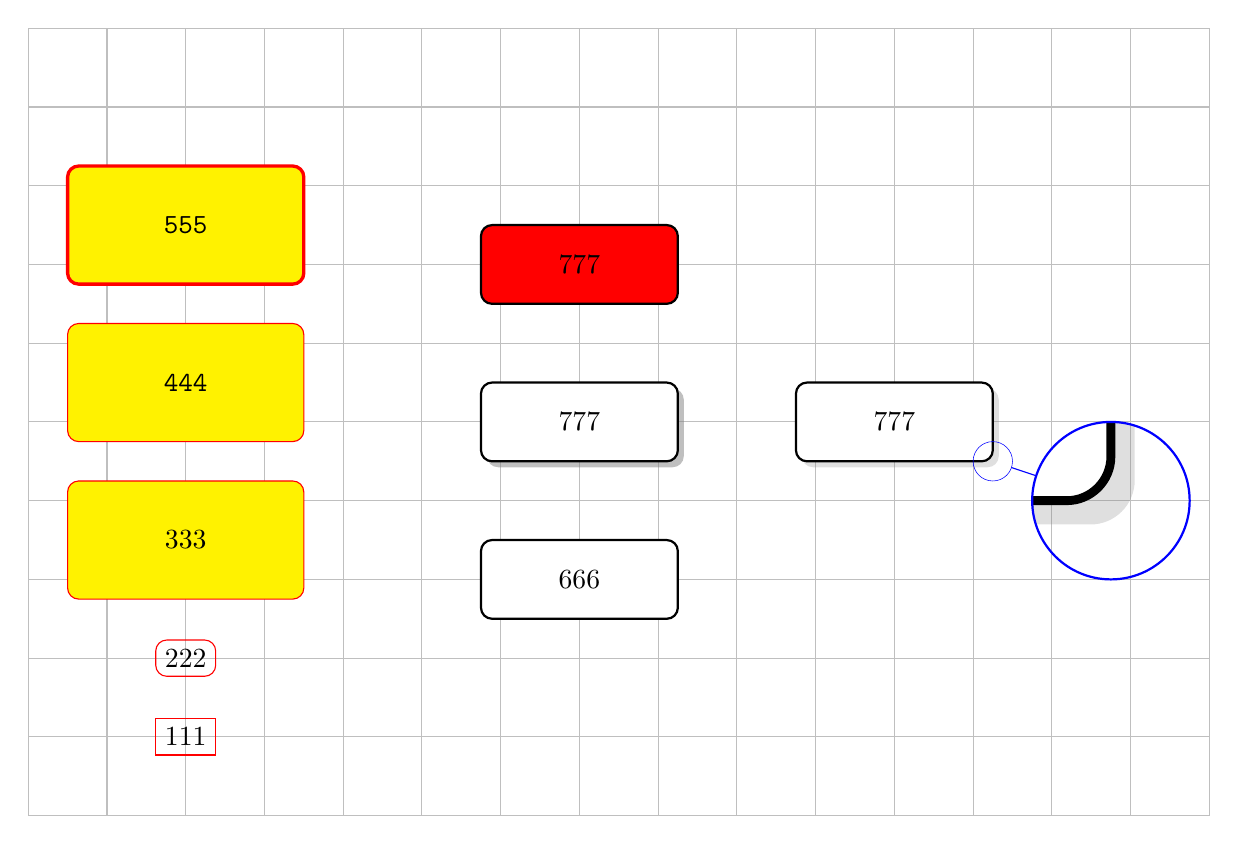
\begin{tikzpicture}
[
mybox/.style={rectangle,draw=black, rounded corners,xshift=1cm,yshift=1cm,minimum width=25mm, thick, minimum height=10mm},
redbox/.style={mybox, fill=red},
spy using outlines={circle, magnification=4, size=3cm, connect spies}
]
\draw[step=1cm,lightgray,thin] (0,0) grid (15,10);

\node[rectangle,draw=red] (a) at (2,1){111};

\node[rectangle,rounded corners,  draw=red] (b) at (2,2){222};

\node[rectangle,rounded corners,  minimum width=30mm, minimum height=15mm, draw=red, fill = yellow] (c) at (2,3.5){333};

\node[rectangle,rounded corners,  minimum width=30mm, minimum height=15mm, draw=red, fill = yellow, font=\ttfamily\bfseries] (d) at (2,5.5){444};

\node[rectangle,rounded corners,  minimum width=30mm, minimum height=15mm, draw=red, very thick, fill = yellow, font=\ttfamily\bfseries] (e) at (2,7.5){555};

\node[mybox, fill = white] (f) at (6,2){666};

\node[mybox, fill = white, drop shadow] (g) at (6,4){777};

\node[redbox] (g) at (6,6){777};

\node[mybox, fill = white, drop shadow={opacity=0.25}] (g) at (10,4){777};

\spy [blue, size=2cm] on (12.25,4.5) in node [right] at (12.75,4);

\end{tikzpicture}
\end{document}
 
 
% rectangle, circle, and coordinate are always defined
% rest via shapes library